\section{Process}
\subsection{Overall Roadmap}

In order to obtain a smaller model, less training and running with better performance, we decided to make multiple models and training improvements based on DCGAN\upcite{dcgan} and improve it through multiple sets of experiments.
Figure \ref{roadmap} is the overall technical roadmap for this study.

\begin{figure}
    \begin{center}
    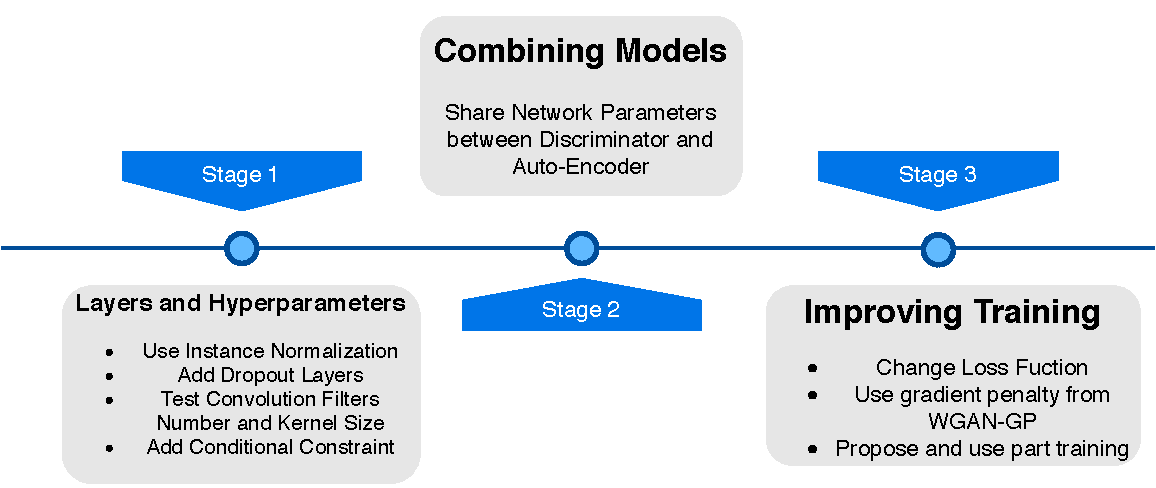
\includegraphics[width=0.48\textwidth]{figures/roadmap.pdf}
    \caption{Overall technical Roadmap}
    \label{roadmap}
    \end{center}
\end{figure}


\subsection{Research Process}

In the previous model adjustments, we conducted several comparative tests to select suitable
hyperparameters.

Figure \ref{norm_bach} and Figure \ref{norm_instance} show the results of the model after two epochs (about 5500 iterations per epoch) using batch normalization and instance normalization respectively.
It can be seen that the image quality is under the same training amount after instance normalization.
There is a certain improvement, which means that the convergence speed of the model is faster.

\begin{figure}
    \begin{center}
    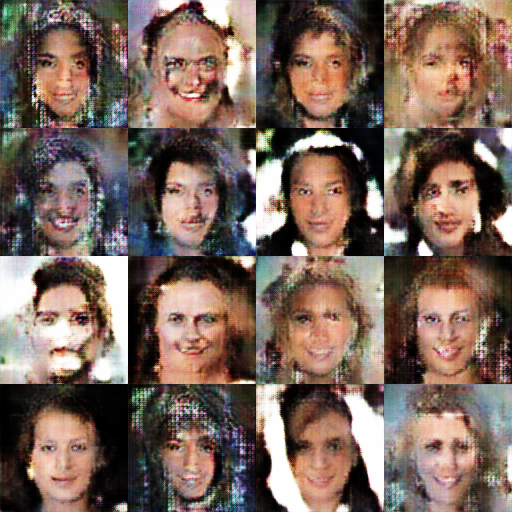
\includegraphics[width=0.48\textwidth]{figures/result_norm_batch.png}
    \caption{Test result using Batch Normalization after 2 epoch}
    \label{norm_bach}
    \end{center}
\end{figure}

\begin{figure}
    \begin{center}
    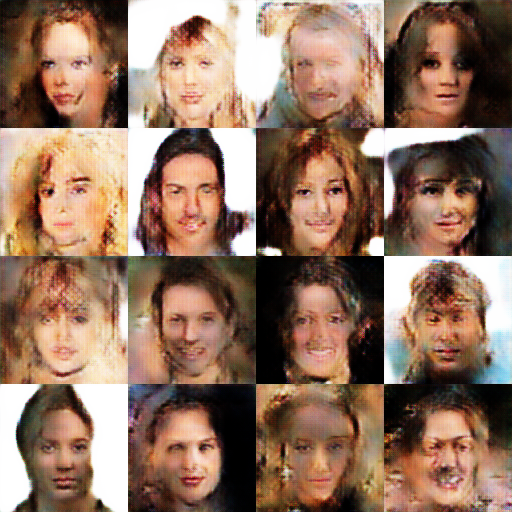
\includegraphics[width=0.48\textwidth]{figures/result_norm_instance.png}
    \caption{Test result using Instance Normalization after 2 epoch}
    \label{norm_instance}
    \end{center}
\end{figure}

In addition, we tested the effects of convolution kernel size and number of convolution filters on model performance and model volume.
Fig.\ref{conv_filter_16}, Fig.\ref{conv_filter_24}, and Fig.\ref{conv_filter_32} are convolution filters using 16 times, 24 times, and 32 times, respectively and the output results are completed after 15 epochs.
It can be seen that after the number of convolution filters is lowered, the image quality does not decrease markedly under the same training amount.
In order to reduce the volume of the model to achieve the purpose of reducing the cost of use, we finally chose a 16 times the number of convolution filters.

\begin{figure}
    \begin{center}
    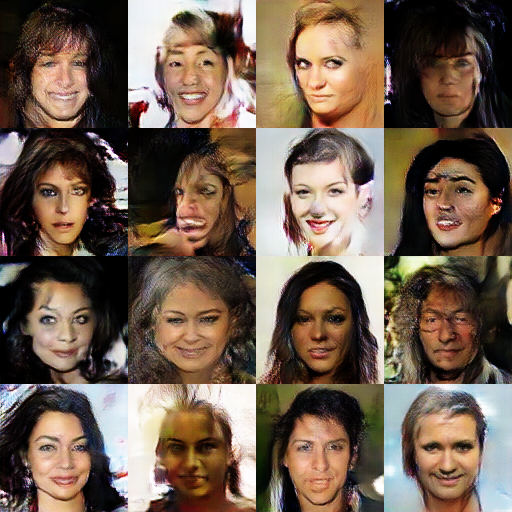
\includegraphics[width=0.48\textwidth]{figures/result_conv_filter_16.png}
    \caption{Test result using 16x convolution filter after 15 epoch}
    \label{conv_filter_16}
    \end{center}
\end{figure}

\begin{figure}
    \begin{center}
    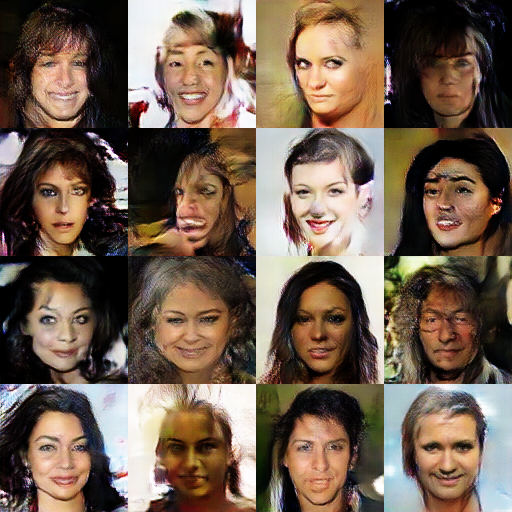
\includegraphics[width=0.48\textwidth]{figures/result_conv_filter_24.png}
    \caption{Test result using 24x convolution filter after 15 epoch}
    \label{conv_filter_24}
    \end{center}
\end{figure}

\begin{figure}
    \begin{center}
    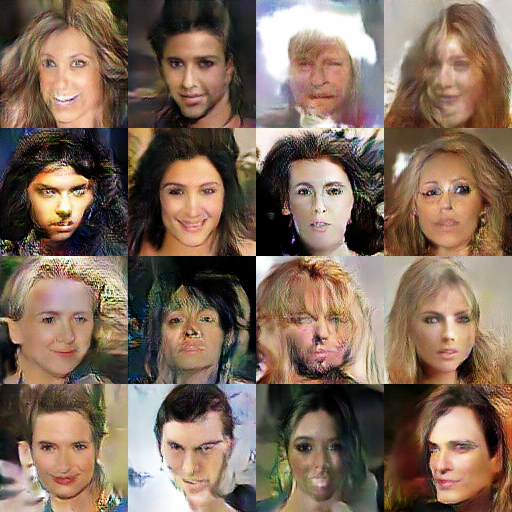
\includegraphics[width=0.48\textwidth]{figures/result_conv_filter_32.png}
    \caption{Test result using 32x convolution filter after 15 epoch}
    \label{conv_filter_32}
    \end{center}
\end{figure}

Figure \ref{conv_kernel_5} and \ref{conv_kernel_3} show the results of the fourth epoch of the convolution kernel (or transposed convolution kernel) of 5×5 size and 3×3 size,
    respectively, under a 16-fold number convolution filter.
It can be seen that switching from a 5×5 size convolution kernel to a 3×3 size,
    the image quality is degraded within an acceptable range, so we chose a 3×3 size convolution kernel.

\begin{figure}
    \begin{center}
    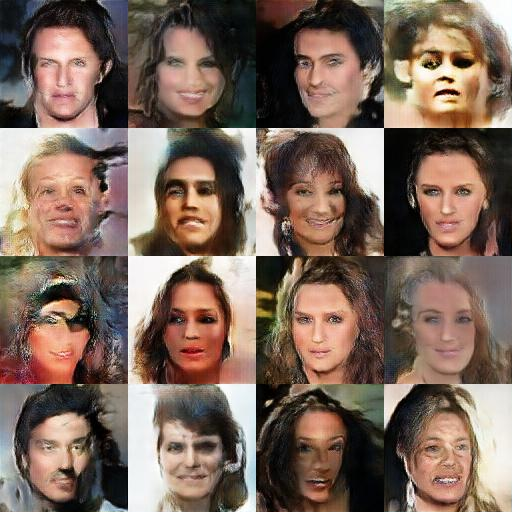
\includegraphics[width=0.48\textwidth]{figures/result_conv_kernel_5.png}
    \caption{Test result using 5×5 size convolution kernel after 4 epoch}
    \label{conv_kernel_5}
    \end{center}
\end{figure}
\begin{figure}
    \begin{center}
    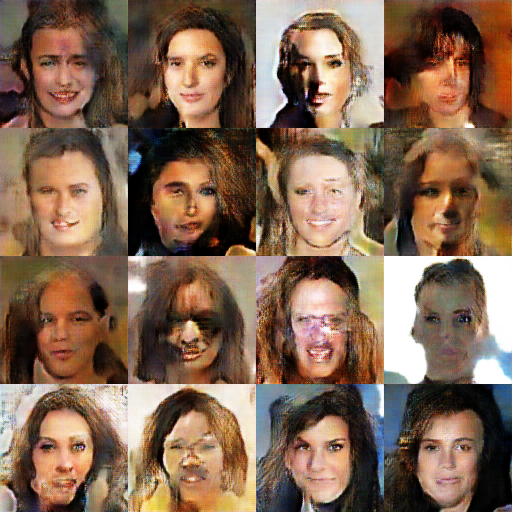
\includegraphics[width=0.48\textwidth]{figures/result_conv_kernel_3.png}
    \caption{Test result using 3×3 size convolution kernel after 4 epoch}
    \label{conv_kernel_3}
    \end{center}
\end{figure}


\subsection{Model Overview}

After the above research, we finally obtained the conditional facial image generation and adjustment model based on GAN\upcite{gan},
    which is a method of facial image generation and adjustment using machine learning (as shown in Figure \ref{smliegan}).

\begin{figure}
    \begin{center}
    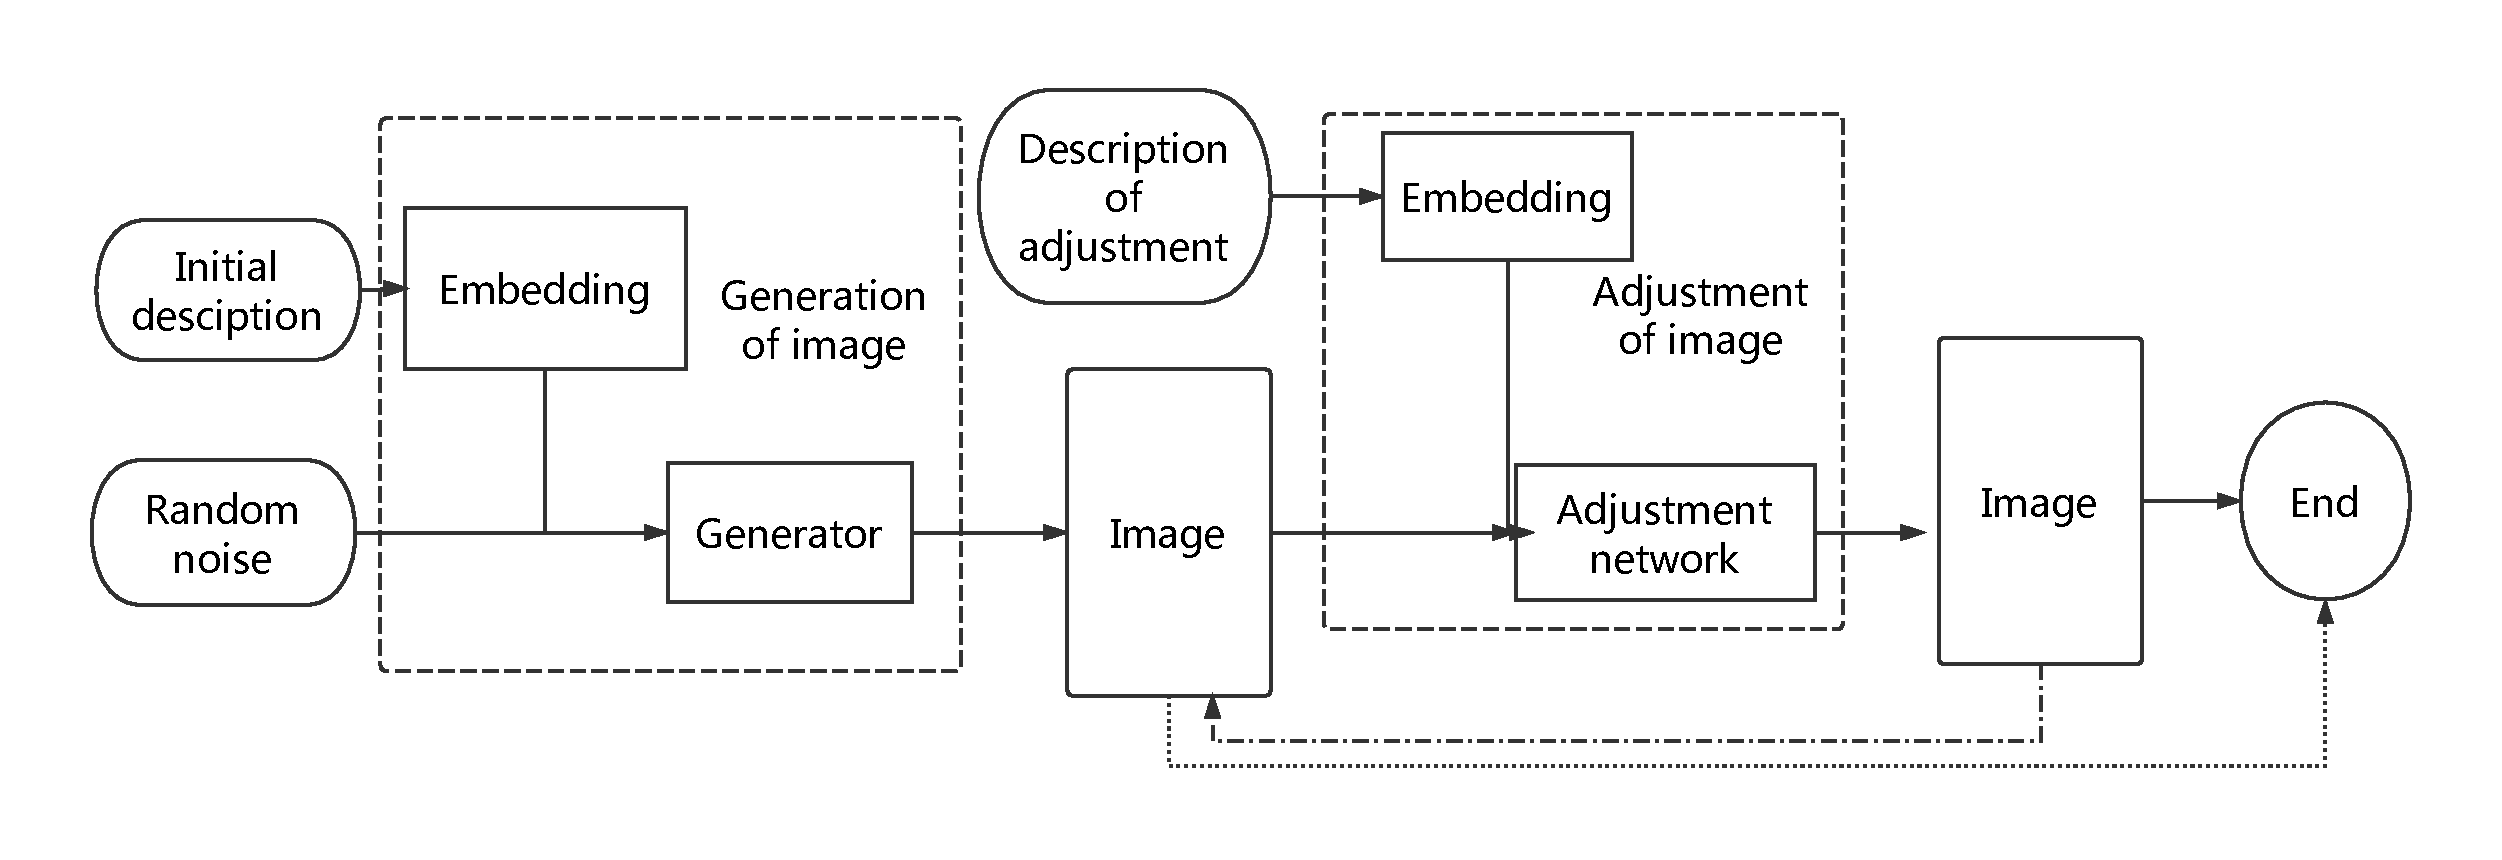
\includegraphics[width=0.48\textwidth]{figures/model.pdf}
    \caption{The Model of SmileGAN}
    \label{smliegan}
    \end{center}
\end{figure}

The model consists of a generative confrontation network and a auto-encoder network.
The main components in the network are the encoder and the decoder and the two networks share the network parameters of the encoder.
In this model, the generator generates a facial image from the noise and face attribute conditions and then combines the original image with the new face attribute condition to obtain a new image by adjusting the network.


\subsection{Decoder and Encoder}

The main component encoder and decoder are used for the conversion of feature vectors and images.
An encoder is used to extract features from an image.
Using a convolution method, starting from an image of 128×128×3 (height × width × channels),
    the convolution operation with step size is continuously performed to extract features while reducing the image dimension.After each convolution operation,
    normalization, activation, and Dropout\upcite{dropout} are performed in order to extract features from the image as a whole to the local.

The convolutional layer uses a convolution kernel size of 5×5.
The filter is incremented from the 16th layer and the step size is set to 2 so the image dimension is reduced when the feature is extracted,
    and the network is lowered with lower calculation amount.
Since the gradient penalty proposed in WGAN-GP\upcite{wgan-gp} is used in the training,
    our normalization layer chose Instance Normalization\upcite{instance}.
To preserve the image for more information, the activation function uses Leaky ReLU with alpha=0.2.
In order to alleviate the occurrence of over-fitting,
    Dropout\upcite{dropout} is used in the training to randomly hide some neurons to reduce the interaction between filters.

The decoder is used to generate an image from the feature vector.
Using the method of transposition convolution, the same number of filters,
    step size, and convolution kernel are symmetrically used with the encoder.
Normalization and activation are performed after each transposition convolution operation.
The normalization layer and the activation function are normalized to the same instance as the encoder and the Leaky ReLU with alpha = 0.2.


\subsection{Generative Adversial Network}

In generative adversarial networks, the model consists of a fully connected layer and a decoder.
The facial attribute condition is combined with random noise to generate an image by transposing convolution.
The discriminator consists of an encoder and a fully connected layer at the bottom,
    and extracts features by convolution and combines them.
The condition determines whether the image comes from the real world and extracts the facial attribute information implied by the image.

The top of the generator is a fully connected network that joins the input facial attribute conditions and the noise (implicit vector) that conform to the normal distribution into a 4×4×n layer feature map.
After the second and fourth convolution, the feature map connected by the facial attribute condition parameter is added,
    and then the image is generated from the global to the local by the decoder layer by layer.
Finally a convolution operation with a step size of 1 and a filter number of 3 is performed and used.
The tanh function is activated to obtain a three-channel color image of 128×128×3 size.
Figure \ref{net_generator} is the graph of generate network structure.

\begin{figure}
    \begin{center}
    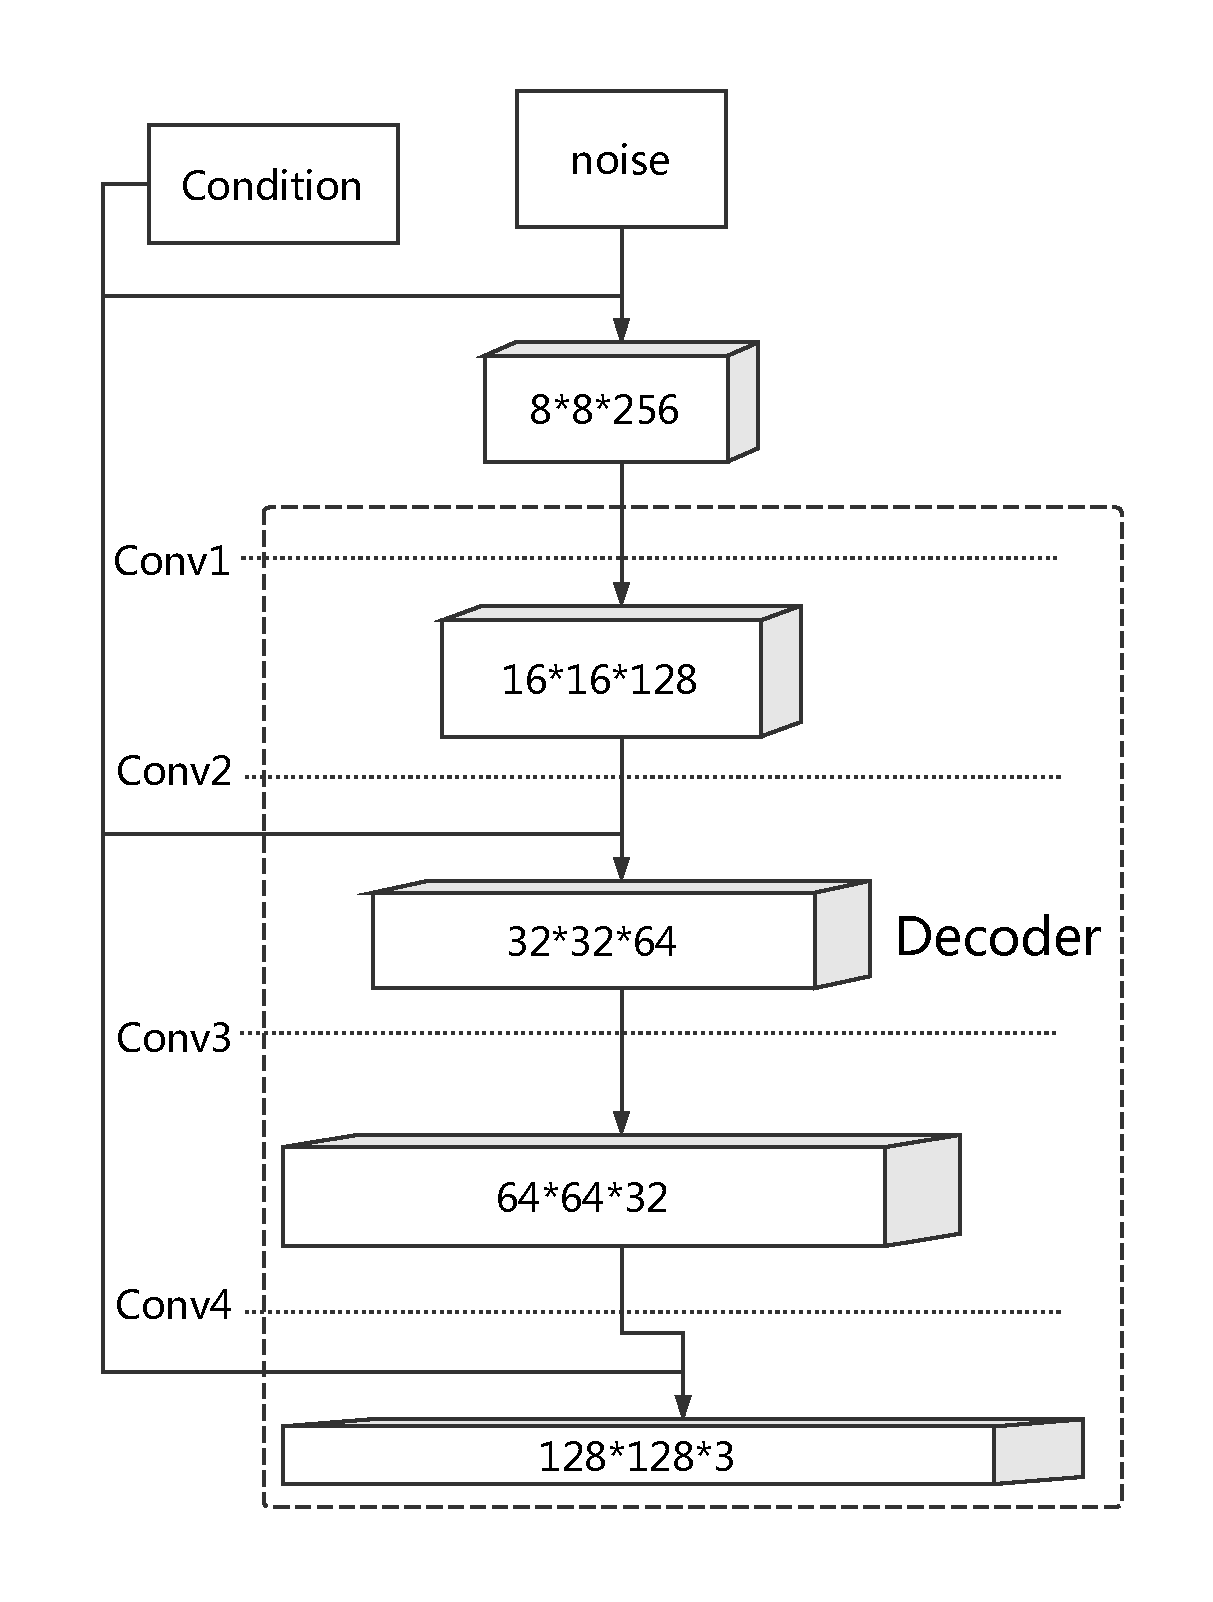
\includegraphics[width=0.48\textwidth]{figures/net_generator.pdf}
    \caption{The Generator Network Structure of SmileGAN}
    \label{net_generator}
    \end{center}
\end{figure}

The top of the discriminator is an encoder that extracts the feature vector of 4×4×n size from the input image.
Finally, the feature vectors are fully connected.
On the one hand, the vector is connected to the dimension 1.
The Sigmoid activation function is used to normalize the result to 0~1,
    which indicates the possibility that the image comes from real data.
On the other hand, connected to the same dimension as the feature vector,
    the latent facial attribute information is extracted,
    and the result is also normalized to 0~1 using the Sigmoid activation function,
    thereby indicating the possibility that the image has these facial attributes.
Figure \ref{net_discriminator} is the graph of generate network structure.

\begin{figure}
    \begin{center}
    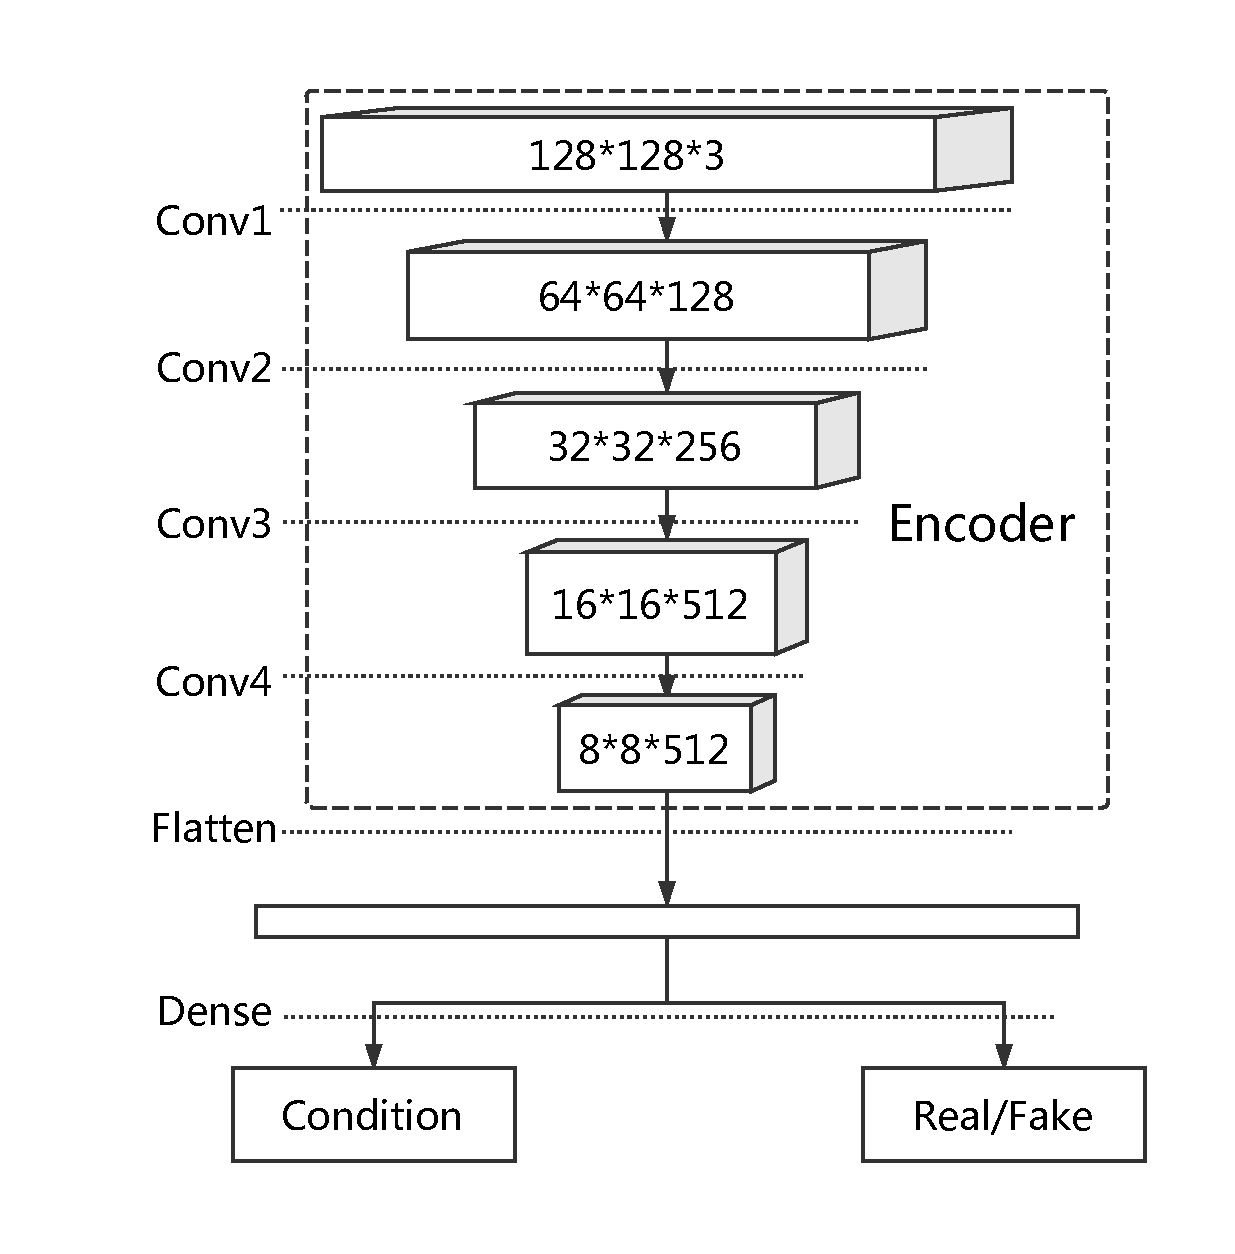
\includegraphics[width=0.48\textwidth]{figures/net_discriminator.pdf}
    \caption{The Discriminator Network Structure of SmileGAN}
    \label{net_discriminator}
    \end{center}
\end{figure}

For the discriminator loss, since the Sigmoid is used to activate the output,
    in order to ensure that the neuron parameters in the network layer are not too large or too small leading to model out of balance,
    we limit the loss of the discriminator output to 0.02~0.98.
Since the discriminator not only outputs whether the image is from the real world but also contains the facial attribute information implied by the image,
    it includes the GAN loss and the conditional judgment loss.
We expect the discriminator to be as close as possible to the true image discrimination result as close as 0.98,
    and the discriminant result from the generator image is as close as possible to 0.02.
Similarly, it is desirable that the facial attribute information output by the discriminator is as consistent as possible with the real data.
Equation \eqref{loss_d_gan}, Equation \eqref{loss_d_a}, and Equation \eqref{loss_d} are the GAN loss, conditional adjustment loss and total loss of the discriminator, respectively.


\begin{equation}
    Loss_{D-GAN}(D,G)=
    \mathbb{E}_{y\thicksim P(data)}[(0.98-D(y))^2]+
    \mathbb{E}_{c,z\thicksim P(fake)}[D(G(c,z))^2]
    \label{loss_d_gan}
\end{equation}


\begin{equation}
    Loss_{A}(A)=
    \mathbb{E}_{c,y\thicksim P(data)}[(c-A(y))^2]
    \label{loss_d_a}
\end{equation}

\begin{equation}
    Loss_{D}(A,D,G)=
    Loss_{D-GAN}(D,G)+
    Loss_{A}(A)
    \label{loss_d}
\end{equation}

We add an mean absolute error to the generator's loss function expecting the model to make the overall color and layout of the generated image more realistic with the diversity of GAN's generation results.
We expect the result of the generator to make the discriminator result close to 0.98 as much as possible, which is consistent with the real image.
Therefore, the loss function of the generator is divided into GAN loss and the mean absolute error loss.
Equation \eqref{loss_g_gan}, Equation \eqref{loss_g_l1}, and Equation \eqref{loss_g} are the GAN loss, mean absolute error loss and total loss of the generator, respectively.
The $\lambda$ in the total loss in the experiment is 0.02.

\begin{equation}
    Loss_{G-GAN}(A,D,G)=
    \mathbb{E}_{c,z\thicksim P(fake)}[(0.98-D(G(c,z)))^2]+
    \mathbb{E}_{c,z\thicksim P(fake)}[(c-A(G(c,z)))^2]
    \label{loss_g_gan}
\end{equation}

\begin{equation}
    Loss_{G-L1}(G)=
    \mathbb{E}_{c,y,z\thicksim P(data)}[|y-G(c,z)|]
    \label{loss_g_l1}
\end{equation}

\begin{equation}
    Loss_{G}(A,D,G)=
    Loss_{G-GAN}(A,D,G)+
    \lambda Loss_{G-L1}(G)
    \label{loss_g}
\end{equation}

Our goal is to minimize the loss function of the generator and the discriminator, so the optimization goal of the generator against the network is Equation \eqref{gan_target}

\begin{equation}
    GAN^*=\arg \min_{A,D} \max_{G}Loss_{D}(A,D,G)+Loss_{G}(A,D,G)
    \label{gan_target}
\end{equation}


\subsection{Auto-Encoder Network}
The auto-encoder network is composed of a decoder, an encoder, a plurality of shortcut channels and a combined channel of adjustment conditions.
The network uses an encoder to extract features from the global to the detail layer by layer and transmits each layer feature to the decoder network through a shortcut channel so that each layer of the network does not need to carry all the information of the image.
The network uses the decoder to combine the original features and adjustment conditions of the image from the detail to the global step by step to generate an image.

Figure \ref{net_auto-encoder} is the graph of generate network structure.

\begin{figure}
    \begin{center}
    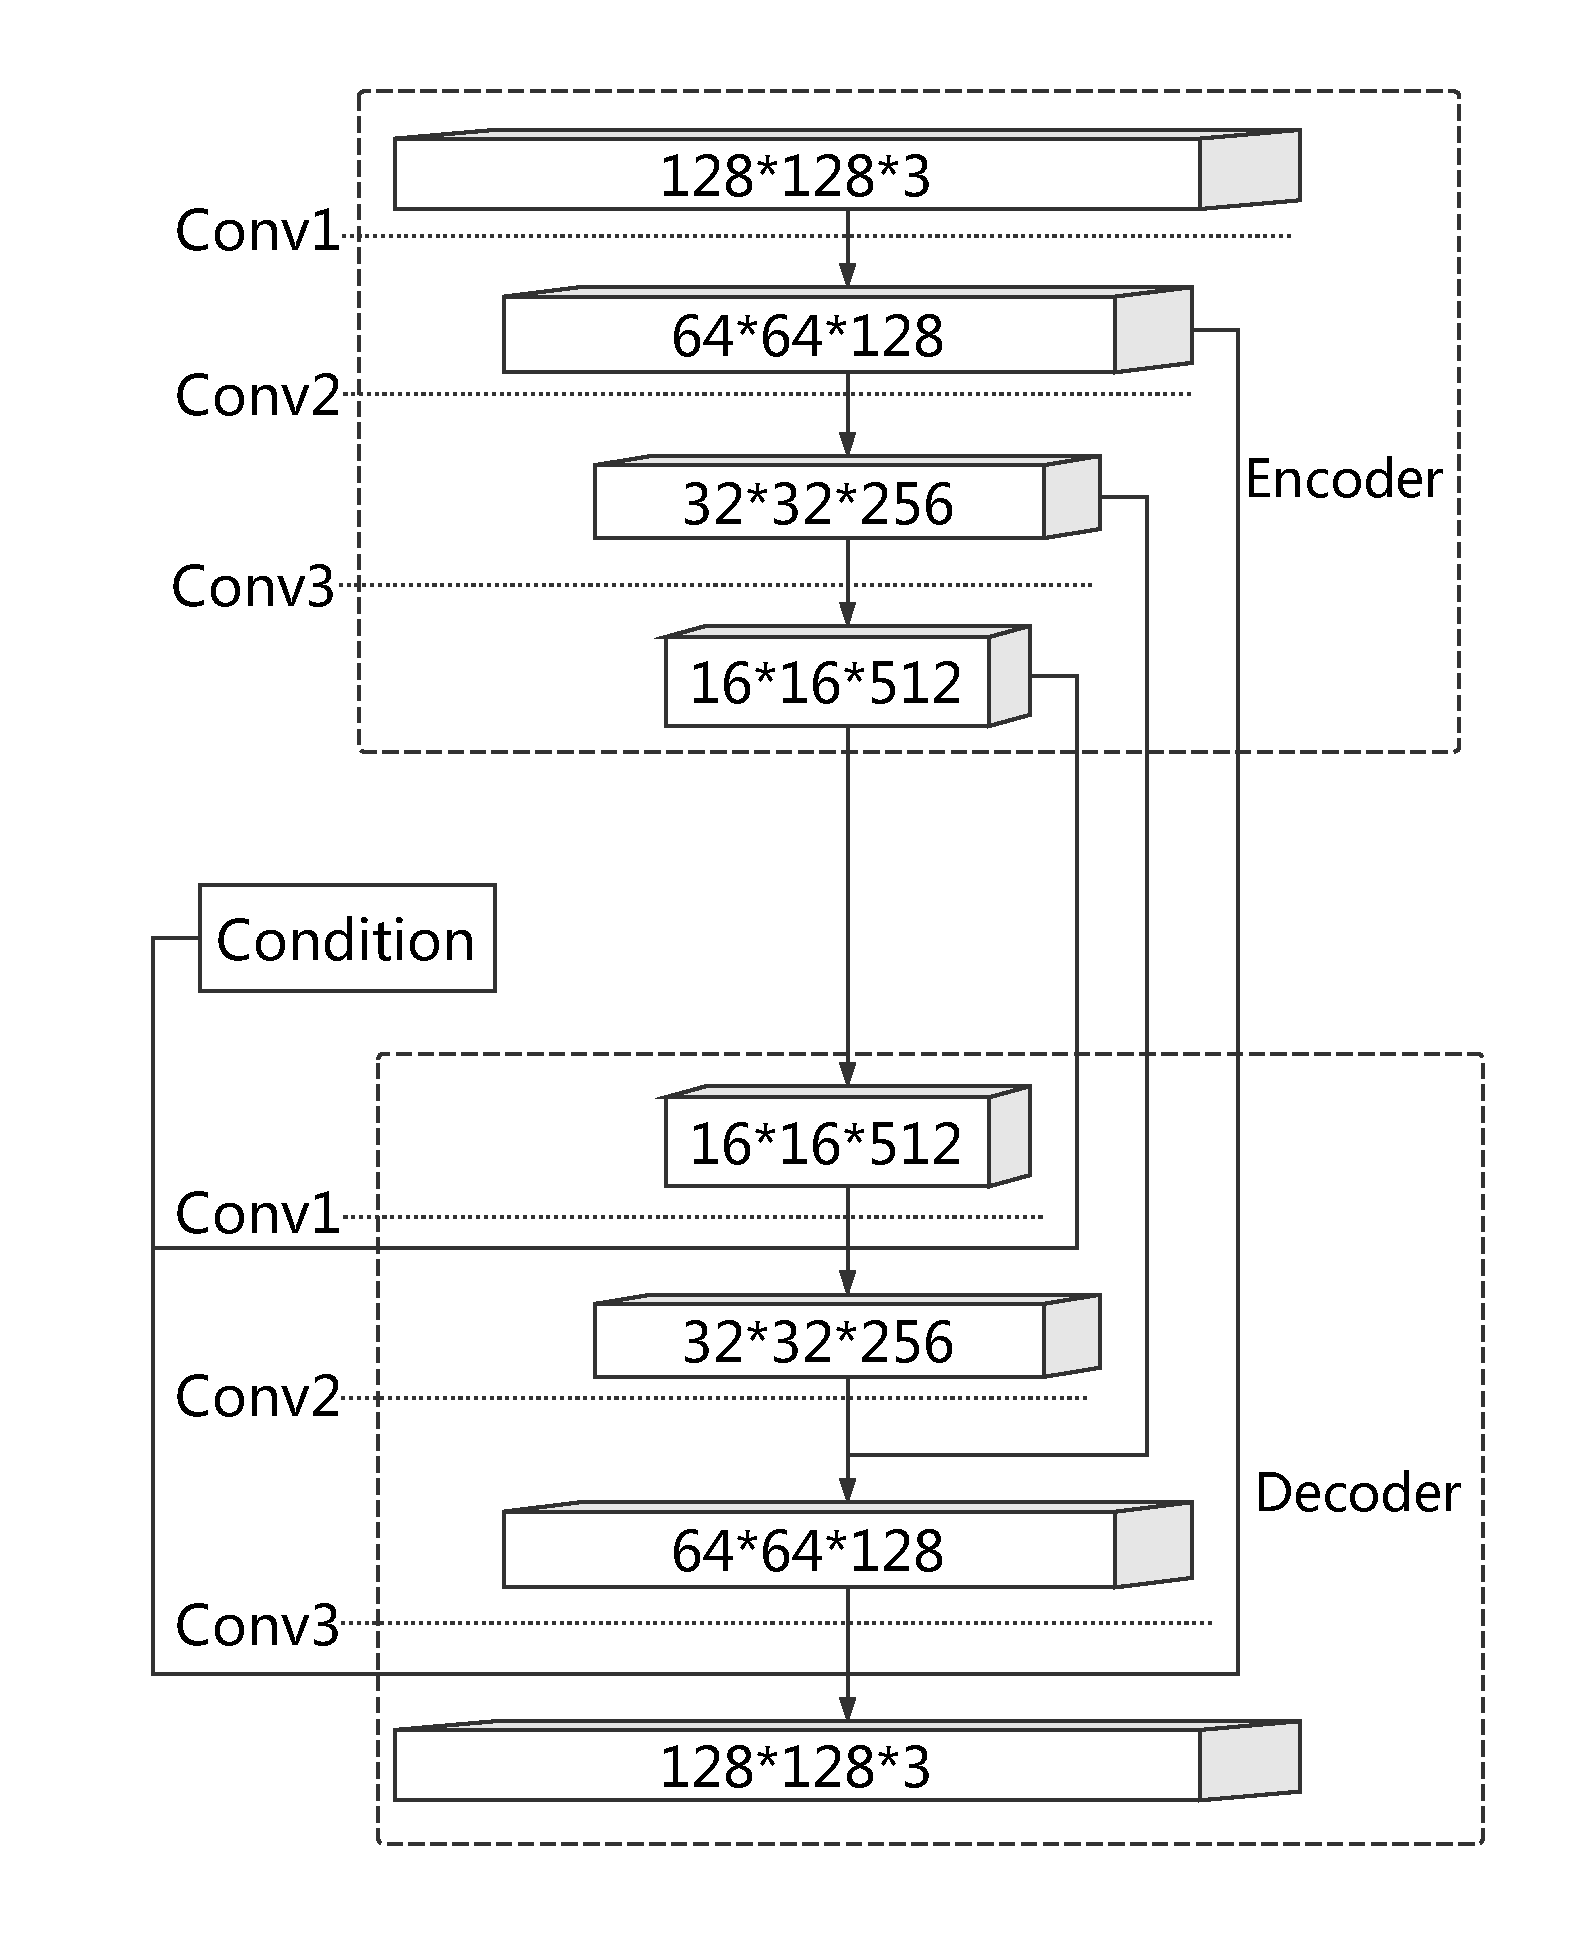
\includegraphics[width=0.48\textwidth]{figures/net_auto-encoder.pdf}
    \caption{The Auto-Encoder Network Structure of SmileGAN}
    \label{net_auto-encoder}
    \end{center}
\end{figure}

In a auto-encoder network, the parameters of the decoder are independent of the decoder parameters in the GAN and the encoder parameters are shared with the GAN.
We use GAN loss and absolute mean error as a loss function for the auto-encoder network.
Equation \eqref{loss_u_gan}, Equation \eqref{loss_u_l1}, and Equation \eqref{loss_u} are the GAN loss, mean absolute error loss and total loss of the auto-encoder, respectively.

\begin{equation}
    Loss_{U-GAN}(A,D,U)=
    \mathbb{E}_{c,y\thicksim P(data)}[(0.98-D(U(c,y)))^2]+
    \mathbb{E}_{c,y\thicksim P(data)}[(c-A(U(c,z)))^2]
    \label{loss_u_gan}
\end{equation}

\begin{equation}
    Loss_{U-L1}(U)=
    \mathbb{E}_{c,x,y\thicksim P(data)}[|y-U(c,z)|]
    \label{loss_u_l1}
\end{equation}

\begin{equation}
    Loss_{U}(A,D,U)=
    Loss_{U-GAN}(A,D,U)+
    \lambda Loss_{U-L1}(U)
    \label{loss_u}
\end{equation}

\subsection{Model Training}
There are two main improvements to the training method of the model:
    applying the gradient penalty proposed in WGAN-GP\upcite{wgan-gp} to the discriminator to improve the convergence speed of the model training and the stability of the model;
    using the part training that proposed by us enables the network to adjust the previous network layer more effectively and speed up the convergence.

The specific operation of the part training proposed by us is as follows: the network layer parameters that need to be trained in the model are grouped according to the function and the number of parameters.
When training each group of parameters, other parameters are fixed and only the parameters in the group are back-propagated.
In practice, for the overall effect of the model, we generally cross the overall model training and part training in a certain proportion.
We set up separate optimizers for each set of parameters.
Although this will take up more memory for the training device, it can reduce the CPU's burden that the optimizer frequently switches the optimization target and reconstructs the model.